\chapter{Este capítulo es una ayuda-memoria}


Acá quiero describir paso por paso lo que hago en el análisis detalladamente en cada paso. Esto es de uso personal y no está pensado para que otra persona lo siga todavía.

	S\subsubsection{Cortes a los datos}
		\begin{itemize}
			\item ($2$) Number of Selected Stations > 2
			\item ($22$) Estimation and Reconstruction compatibles >0
			\item ($23$) Is T5 > 0
			\item ($43$) Number ot neighbours in the hottesk tank > 5 or 6. Depende del rango de energía. Este es el filtro de 5t5 o 6t5.
			\item ($44$) Flag with $43$ > 0
			\item ($48$) Bad period: 1. Si es 1 es un good period.
 		\end{itemize}

\section{Análisis de los parametros del  clima}

\subsection{Preparando los datos}
	 El archivo del datos tiene 48 columnas. La información sobre que es cada columna está en \url{http://ipnwww.in2p3.fr/~augers/AugerProtected/herald.php}.   Los datos que necesito del archivo de los eventos son estos:
			\begin{enumerate}
				\item (\$8)   UTC                  	: unix time 
				\item (\$4)   Phi                  	: angular value of $\phi$, 
				\item (\$3)   Theta                	: declinación
				\item (\$14)  Ra                   	: Ascensión recta
				\item (\$12)  S1000 sin corregir   	: Si corregir por el clima
				\item (\$47)  S38\_w                : Corregida por el clima, en el 2017 es $-1$
				\item (\$38)  Energy         		:
				\item (\$43)  Tanks                	: 
				\item (\$37)  S1000 con correccion 	: En el 2017 vale $-1$.
			\end{enumerate}

	Para el caso del archivo del clima tiene 12 columnas y la información de cada columna \url{http://auger.uis.edu.co/data/private.html}. Los datos se toman cada 5 minutos. Para los análisis necesitamos,

			\begin{enumerate}
				\item utc time
				\item Temperatura
				\item Presión
				\item rho
				\item rho media durante las 24 horas anteriores
				\item 6t5 (Está sumado durante 5 min, hay que dividir por 5 para el número posta)
				\item 5t5 (Está sumado durante 5 min, hay que dividir por 5 para el número posta)
				\item iw: bad weather
					\begin{itemize}
						\item 0: es lo que se registró
						\item 1: se interpoló con datos menos de 3 horas
						\item 4: Mayor a 3 horas.
					\end{itemize}
				\item bad period: 0 si estaba mal, 1 estaba bien
			\end{enumerate}

	Para cotinuar con el  análisis, tenemos que agregar dos columnas por nuestra cuenta
			\begin{enumerate}
				\item[10.] Densidad atrasada en dos horas
				\item[11.] Densidad media 12 horas antes y 12 horas después
			\end{enumerate}
		Para la densidad atrasada 2 horas, tengo que guardar la densidad de ahora e imprimirla dos horas despues


		Para la segunda parte, centrar alrededor de 24, necesito mandar lo de ahora 12 horas atrás.

	\subsubsection{Que hice de esto hasta ahora}

	Preparé el archivo del clima con las 11 columnas para todo el rango de  tiempo (2004 $\rightarrow$ 2019 incluido). 	Para los datos de eventos del 2019 , consideré solo los datos a partir de $1388910508$, antes tienen una tasa rara de eventos que tengo que preguntar.


	\subsection{Agregar a cada evento el clima}

	\subsection{Haciendo el ajuste}


	Considerando 


	\subsection{Problemas que tuve con el ajuste}

	\subsubsection{Tasa de eventos rara para AllTriggers ICRC 2019}
	\begin{figure}[htbp]
		\centering
		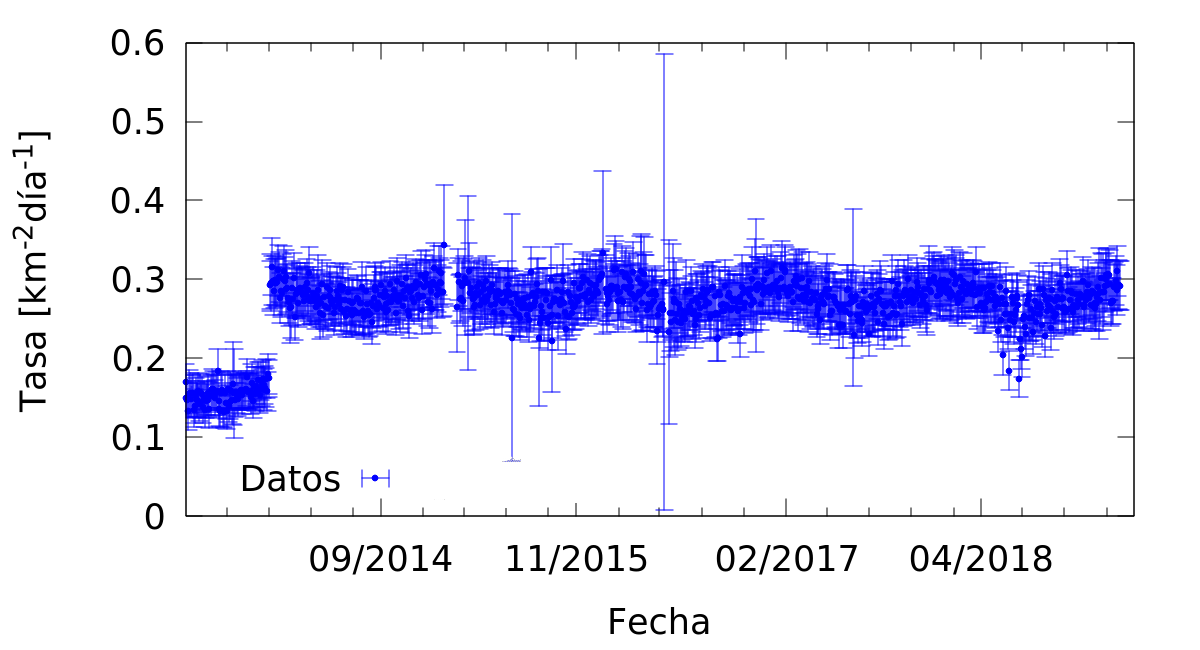
\includegraphics[width=\textwidth]{../Apendice/draft_s38_1EeV_weather_for_reconstruction.png}
		\caption{Hay una tasa de eventos baja en un rango de tiempo, esta media coincide con el main array.}
		\label{fig:tasarara}
	\end{figure}